% ==============================================================================
% MASTER DRIVER FILE: [CF01] The Physics of Governance (v2.1)
% ==============================================================================
\documentclass[11pt, a4paper]{article}

% --- 1. PACKAGES ---
\usepackage[utf8]{inputenc}
\usepackage[T1]{fontenc}
\usepackage{geometry}
\geometry{margin=1in}
\usepackage{graphicx}
\usepackage{amsmath}
\usepackage{amssymb}
\usepackage{amsthm}
\usepackage{booktabs}
\usepackage{tabularx}
\usepackage{float}
\usepackage{hyperref}
\usepackage{caption}
\usepackage{microtype}
\usepackage{xcolor}
\usepackage{tcolorbox} 

% --- 2. GOVERNANCE COLOR PALETTE (CRITICAL FIX) ---
% These definitions prevent the "Undefined Color" crash in the figures.
\definecolor{GovRed}{rgb}{0.8, 0.2, 0.2}
\definecolor{GovBlue}{rgb}{0.2, 0.4, 0.8}
\definecolor{GovGold}{rgb}{0.8, 0.6, 0.1}
\definecolor{GovGray}{rgb}{0.5, 0.5, 0.5}

% --- 3. PHYSICS ENGINE (TIKZ) ---
% These libraries are required for the "Twin" diagrams to render natively.
\usepackage{tikz}
\usepackage{pgfplots}
\pgfplotsset{compat=1.18}
\usetikzlibrary{calc, positioning, arrows.meta, decorations.pathmorphing, patterns, fadings, shadows, backgrounds, fit, shapes}

% --- METADATA ---
\title{\textbf{Volume I: The Physics of Governance:}\\Thermodynamic Limits of Autonomous Agents}
\author{
    \textbf{Matthew A. Davis} \\[0.3em]
    \small \textit{The Unified Field Theory of Autonomous Governance Project} \\[0.3em]
    \footnotesize \texttt{m@ontoramp.com} $\,\cdot\,$ \url{linkedin.com/in/mdavis01} \\[0.3em]
    \footnotesize ORCID: 0009-0000-4309-3874
}
\date{August 2026}

\newcommand{\Ge}{G_E}
\newcommand{\Gi}{G_I}
\newcommand{\Wgov}{W_{Gov}}
\newcommand{\Vctx}{V_{Context}}
\newcommand{\ReCtx}{Re_{Ctx}}
\newcommand{\OmegaStab}{\Omega_{Stability}}

% --- THEOREM ENVIRONMENTS (v2.1) ---
% Unnumbered by design: adds no new citable number to the frozen label set.
\newtheorem*{fundamentaltheorem}{Fundamental Theorem of AI Governance}

\begin{document}

\maketitle

\begin{abstract}
The deployment of autonomous agents in high-stakes enterprise environments is currently constrained by a fundamental misunderstanding of alignment. We propose that "Governance" is not a policy layer but a thermodynamic function. By modeling the agent as a closed system subject to the Second Law of Thermodynamics, we demonstrate that "Drift" ($\Gi$) is equivalent to entropy and "Alignment" ($\Ge$) requires a continuous expenditure of kinetic work ($\Wgov$). We derive the \textit{Governance Jeans Instability}, proving that because self-attention scales quadratically ($O(N^2)$), the density of the system prompt must scale non-linearly to prevent identity collapse. We conclude by defining the "Gibbs Governance Criterion," offering a unified potential function that predicts spontaneous drift based on the enthalpy of the constitution and the entropy of the context.
\end{abstract}

% --- KEYWORDS ---
\vspace{1em}
\noindent\textbf{Keywords:} AI Governance, Thermodynamics of Computation, Jeans Instability, Context Collapse, Transformer Architecture, Entropy, Gibbs Free Energy.

% --- DATA / CODE AVAILABILITY ---
\vspace{0.5em}
\noindent\textbf{Data and code availability:} This paper contains no datasets or experimental code. The complete \LaTeX{} source, including all TikZ figure sources and the bibliography, is maintained at \url{https://github.com/MatthewDavisAIArchitect/pog-vol1-paper} (tag \texttt{v2.1}) and archived on Zenodo (concept DOI: 10.5281/zenodo.18645592).

% --- TABLE OF CONTENTS ---
\vspace{1em}
\begin{center}
\begin{tcolorbox}[colback=white, colframe=black, title=\textbf{Contents}]
\makeatletter
\@starttoc{toc}
\makeatother
\end{tcolorbox}
\end{center}
\vspace{2em}

% ==============================================================================
% SECTION 1: THE THERMODYNAMICS OF INTENT
% ==============================================================================
\section{The Thermodynamics of Intent: Defining $\Ge$ and $\Gi$}
\label{sec:thermodynamics}

The fundamental error in the current deployment of autonomous agents is the assumption of deterministic compliance. In classical software engineering, a function $f(x)$ yields a predictable output $y$ with zero variance. In generative artificial intelligence, the output is probabilistic, governed by a high-dimensional vector space where "correctness" is merely a region of high probability, not a binary state.

Therefore, we must reject the biological metaphor of "teaching" the model and adopt the physical metaphor of \textit{constraining} it. We model the enterprise interaction layer as a closed thermodynamic system seeking to maintain a specific state of order (Alignment) against the natural pressure of disorder (Entropy).

To quantify this, we establish the \textbf{Nomenclature of Governance Thermodynamics} (Table \ref{tab:nomenclature}), defining the variables required to calculate the stability of an autonomous agent.

% --- TABLE: NOMENCLATURE (v2.0 REMEDIATED) ---
\begin{table}[H]
\centering
\caption{\textbf{Nomenclature of Governance Thermodynamics (v2.0).}}
\label{tab:nomenclature}
\renewcommand{\arraystretch}{1.5}
\begin{tabularx}{\textwidth}{@{}c l X@{}}
\toprule
\textbf{Symbol} & \textbf{Variable} & \textbf{Thermodynamic Properties} \\
\midrule
$\Ge$ & \textbf{The Constitution} & \textbf{The Enthalpy (Binding Energy).} \newline
\textit{Operational Function:} Acts as the gravitational center ($H$) to resist entropy. \newline
\textit{Failure Mode:} \textbf{Identity Dissolution.} If $T\Delta S > \Delta H$, the mass collapses. \\
\midrule
$\Gi$ & \textbf{Implicit Drift} & \textbf{The Entropy (Disorder).} \newline
\textit{Operational Function:} The stochastic pressure of the environment. \newline
\textit{Failure Mode:} \textbf{Turbulence.} Unchecked drift leads to hallucination ($\ReCtx > Re_{Crit}$). \\
\midrule
$\Wgov$ & \textbf{Governance Work} & \textbf{The Kinetic Expenditure.} \newline
\textit{Operational Function:} The active energy (Joules/Bit) required to filter noise. \newline
\textit{Failure Mode:} \textbf{Insolvency.} When cost of alignment exceeds available compute. \\
\bottomrule
\end{tabularx}
\end{table}

\subsection{The Vector Space of Alignment}

In this framework, "Alignment" is not a sentiment; it is a vector orientation. An agent is "aligned" when its output vector is parallel to the enterprise's intent vector. However, as the agent interacts with users, external data, and retrieved context (RAG), it absorbs energy from the environment. This absorption creates an orthogonal force we define as \textit{Drift}.

We formally define the total operational state of an autonomous agent, denoted as $\Psi$, not as a singular personality, but as the superposition of two distinct vector fields:

\begin{equation}
    \label{eq:total_state}
    \Psi_{Agent}(t) = \Ge \cdot \hat{i} + \Gi(t) \cdot \hat{j}
\end{equation}

\noindent
Where:
\begin{itemize}
    \item $\Ge$ (\textbf{Explicit Governance}) is the immutable core identity—the "Constitution" of the firm. It acts as the system's Internal Energy ($U$). In an ideal state, it is time-independent ($\frac{d\Ge}{dt} = 0$).
    \item $\Gi$ (\textbf{Implicit Drift}) is the "Contextual Entropy." It represents the cumulative noise introduced by user prompts, conversation history, and stochastic sampling. It is time-dependent and orthogonal to the intent.
\end{itemize}

\subsection{The First Law: Conservation of Intent}

The \textbf{First Law of Governance Dynamics} posits that for an enterprise to remain secure, the closed-loop intent must be conserved across the duration of the session \cite{davis2026}. The divergence of the system state from the constitutional vector must be minimized:

\begin{equation}
    \label{eq:conservation}
    \frac{d\Psi}{dt} = \frac{d\Ge}{dt} + \frac{d\Gi}{dt} \approx 0 \implies \frac{d\Gi}{dt} \to 0
\end{equation}

\noindent
However, autonomous agents operate in open environments. They are subject to the \textbf{Second Law of Contextual Entropy}: as the volume of the Context Window ($\Vctx$) expands, the system's exposure to stochastic noise increases strictly monotonically. The Drift vector $\Gi$ is therefore a function of time and context volume:

\begin{equation}
    \label{eq:drift_entropy}
    \Gi(t) \propto \int_{0}^{t} \Vctx(\tau) \cdot S_{Model} \, d\tau
\end{equation}

\noindent
Where $S_{Model}$ represents the inherent temperature or "creativity" of the model. This equation reveals the hidden danger of long-context interactions: \textbf{Alignment decays as a function of interaction length.}

% ==============================================================================
% SECTION 2: THE GOVERNANCE ENGINE
% ==============================================================================
\section{The Governance Engine: Maxwell's Demon in the Loop}
\label{sec:governance_engine}

% --- FIGURE BLOCK: STATIC TWIN 1 (GOVERNANCE ENGINE) ---
\begin{figure}[t!]
    \centering
    % REPLACEMENT: Static TikZ Twin (Maxwell's Demon)
    \resizebox{0.95\textwidth}{!}{% FILE: figures/Fig01_Governance_Engine.tex
% CONTEXT: Maxwell's Demon (The Classifier Swarm)
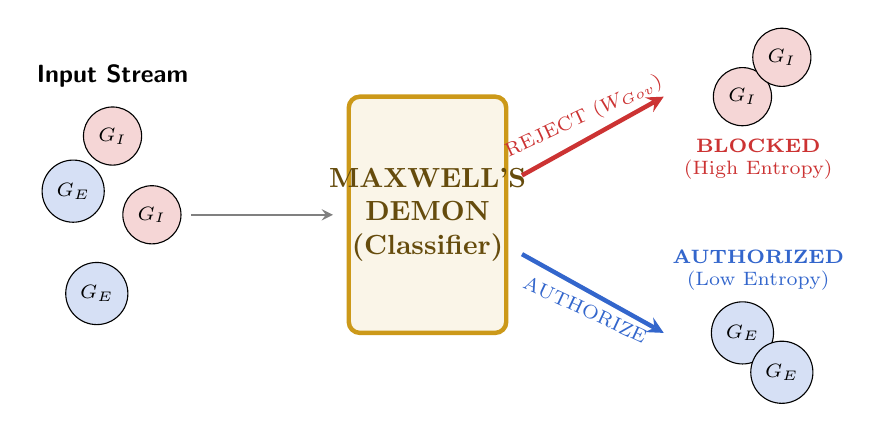
\begin{tikzpicture}[
    font=\sffamily\small,
    >=stealth,
    scale=1.0, transform shape,
    % Styles
    token/.style={circle, draw=black, thin, minimum size=0.6cm, font=\scriptsize},
    high_entropy/.style={token, fill=GovRed!20},
    low_entropy/.style={token, fill=GovBlue!20},
    demon_box/.style={rectangle, draw=GovGold, ultra thick, fill=GovGold!10, minimum width=2cm, minimum height=3cm, rounded corners},
    zone/.style={rectangle, draw=none, fill=gray!5, minimum width=3cm, minimum height=4cm}
]

    % 1. THE INPUT STREAM (Mixed Entropy)
    \node[anchor=south] at (-4, 2) {\textbf{Input Stream}};
    \node[high_entropy] at (-4, 1.5) {$\Gi$};
    \node[low_entropy] at (-4.5, 0.8) {$\Ge$};
    \node[high_entropy] at (-3.5, 0.5) {$\Gi$};
    \node[low_entropy] at (-4.2, -0.5) {$\Ge$};
    
    % Flow Arrow
    \draw[->, thick, gray] (-3, 0.5) -- (-1.2, 0.5);

    % 2. THE DEMON (Governance Engine)
    \node[demon_box] (demon) at (0, 0.5) {};
    \node[text=GovGold!50!black, font=\bfseries, align=center] at (0, 0.5) {MAXWELL'S\\DEMON\\(Classifier)};

    % 3. THE SORTING GATES
    % Upper Gate (Drift/Rejected)
    \draw[->, GovRed, ultra thick] (1.2, 1) -- (3, 2) node[midway, above, rotate=25, font=\scriptsize] {REJECT ($W_{Gov}$)};
    
    % Lower Gate (Aligned/Authorized)
    \draw[->, GovBlue, ultra thick] (1.2, 0) -- (3, -1) node[midway, below, rotate=-25, font=\scriptsize] {AUTHORIZE};

    % 4. THE ZONES
    % Exergonic Zone (Blocked)
    \node[high_entropy] at (4, 2) {$\Gi$};
    \node[high_entropy] at (4.5, 2.5) {$\Gi$};
    \node[text=GovRed, align=center, font=\scriptsize] at (4.2, 1.2) {\textbf{BLOCKED}\\(High Entropy)};

    % Endergonic Zone (Authorized)
    \node[low_entropy] at (4, -1) {$\Ge$};
    \node[low_entropy] at (4.5, -1.5) {$\Ge$};
    \node[text=GovBlue, align=center, font=\scriptsize] at (4.2, -0.2) {\textbf{AUTHORIZED}\\(Low Entropy)};

\end{tikzpicture}}
    \caption[\textbf{The Governance Engine.}]{\textbf{The Governance Engine as thermodynamic filter.} A multi-stage classifier swarm functions as a literary "Maxwell's Demon," mechanically separating incoming data vectors based on their alignment signature. High-entropy inputs---representing chaos, drift ($\Gi$), or adversarial prompting---are shunted to the Blocked Zone. Only low-entropy vectors that conform to the Explicit Governance constitution ($\Ge$) are permitted transition into the Authorized Zone.}
    \label{fig:governance_engine}
\end{figure}

If the natural state of an autonomous system is to drift toward maximum entropy ($\Gi \to \infty$), then the maintenance of alignment ($\Ge$) requires the continuous application of external work. We define this active enforcement layer not as a "guardrail"---a passive barrier---but as a \textbf{Governance Engine}.

Consequently, the "Governance Engine" cannot be merely a software prompt. To achieve the necessary rejection velocity ($v_{reject} > v_{token}$), it must ideally be instantiated as a \textbf{hardware constraint}---a Silicon Photonic Lattice or dedicated ASIC that mechanically filters high-entropy tokens before they reach the model weights.

\subsection{The Thermodynamic Cost of Alignment}

In 1867, James Clerk Maxwell proposed a thought experiment \cite{maxwell1871}: a "demon" controlling a door between two gas chambers, allowing only fast-moving (hot) molecules to pass one way and slow-moving (cold) molecules the other. This action would seemingly violate the Second Law of Thermodynamics by reducing the total entropy of the system without expending energy.

Information Theory later resolved this paradox (via Landauer's Principle) by proving that the act of \textit{sorting} information requires energy \cite{landauer1961}. We apply this principle to Artificial Intelligence. The "Governance Engine" functions as a \textit{computational Maxwell's Demon}. It sits between the User (Input) and the Model (Agent), mechanically separating high-entropy vectors (Ambiguity, Malice, Hallucination) from low-entropy vectors (Constitutional Intent).

As illustrated in \textbf{Figure \ref{fig:governance_engine}}, this separation is not performed by the agent itself---which is subject to drift---but by an external, immutable "Classifier Swarm".

\subsection{The Classifier Swarm Architecture}

The Engine operates on a principle of \textbf{Orthogonal Validation}. We do not ask the Large Language Model (LLM) to auto-regulate, as its own context window is already contaminated by $\Gi$. Instead, we deploy a swarm of lightweight, specialized classifiers (BERT-style encoders or small distilled models) that act as the "Demon's Door".

The work ($\Wgov$) required to maintain alignment is defined as the energy needed to measure the vector $\vec{v}_{input}$ and reject it if it diverges from $\Ge$:

\begin{equation}
    \label{eq:landauer}
    \Wgov \geq \sum_{i=1}^{N} \left( k_B T \ln(2) \cdot I(x_i; \Ge) \right)
\end{equation}

\noindent
Where:
\begin{itemize}
    \item $\Wgov$ is the minimum work required by the Governance Engine to filter the input stream.
    \item $k_B T \ln(2)$ is the Landauer Limit (approx. $2.8 \times 10^{-21}$ Joules per bit at room temperature).
    \item $I(x_i; \Ge)$ is the mutual information \cite{shannon1948} between the input token $x_i$ and the constitutional vector $\Ge$.
\end{itemize}

This inequality dictates that as the precision of the governance requirement ($\Ge$) increases, the energy cost of enforcement scales linearly with the information density of the context. \textbf{Alignment is computationally expensive.} To achieve Zero Drift, the Governance Engine must expend energy proportional to the volume of information flowing through the system.

% ==============================================================================
% SECTION 3: THE HORIZON LIMIT
% ==============================================================================
\section{The Horizon Limit: Information Asymmetry \& Leakage}
\label{sec:horizon_limit}

% --- FIGURE BLOCK: STATIC TWIN 2 (HORIZON LIMIT) ---
% --- FIGURE BLOCK: STATIC TWIN 2 (HORIZON LIMIT) ---
\begin{figure}[t!]
    \centering
    % RESIZED: Reduced by 25% (0.75 -> 0.56)
    \resizebox{0.56\textwidth}{!}{% FILE: figures/Fig02_Horizon_Limit.tex
% CONTEXT: The Containment Field (Superset Topology)
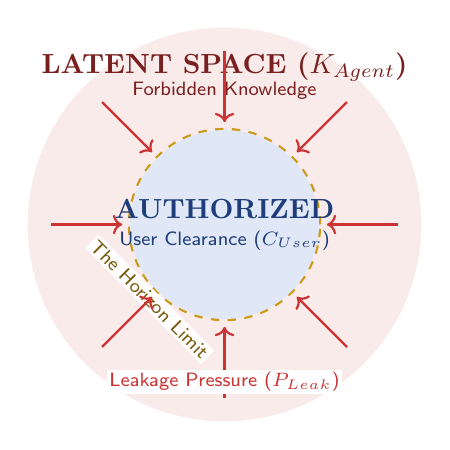
\begin{tikzpicture}[font=\sffamily\scriptsize, scale=1.0, transform shape]

    % 1. THE AGENT'S LATENT OCEAN (The Superset) -> GovRed
    % Represents the vast, unsafe knowledge of the model
    \fill[GovRed!10] (0,0) circle (2.5);
    \node[text=GovRed!60!black, font=\bfseries] at (0, 2.0) {LATENT SPACE ($K_{Agent}$)};
    \node[text=GovRed!60!black] at (0, 1.7) {Forbidden Knowledge};

    % 2. THE HORIZON LIMIT (The Boundary) -> GovGold
    % The hard barrier of the context window/permissions
    \draw[GovGold, ultra thick, dashed] (0,0) circle (1.2);
    \node[text=GovGold!60!black, fill=white, inner sep=1pt, rotate=-45] at (-0.95, -0.95) {The Horizon Limit};

    % 3. THE AUTHORIZED ZONE (The Subset) -> GovBlue
    % The safe, user-visible area
    \fill[GovBlue!15] (0,0) circle (1.2);
    \node[text=GovBlue!60!black, font=\bfseries] at (0, 0.2) {AUTHORIZED};
    \node[text=GovBlue!60!black] at (0, -0.2) {User Clearance ($C_{User}$)};

    % 4. LEAKAGE PRESSURE (Arrows)
    % Visualizes the thermodynamic pressure of the agent trying to leak info in
    \foreach \angle in {0, 45, ..., 315} {
        \draw[->, GovRed, thick] (\angle:2.2) -- (\angle:1.3);
    }
    \node[text=GovRed, fill=white, inner sep=1pt] at (0, -2.0) {Leakage Pressure ($P_{Leak}$)};

\end{tikzpicture}}
    \caption[\textbf{The Horizon Limit.}]{\textbf{The Horizon Limit: Information Asymmetry as a Thermodynamic Boundary.} This diagram visualizes the tension between the model's total latent corpus (``Agent Knowledge'') and the bounded subset of information a specific user is authorized to access (``User Clearance''). The intersection defines the \textbf{Authorized Zone}, a stable, low-entropy state of validated information exchange. The red \textbf{Leakage Zone} represents the high-entropy potential for unauthorized data egress.}
    \label{fig:horizon_limit}
\end{figure}

The "Governance Engine" described in Section \ref{sec:governance_engine} assumes that the threat originates from the user (e.g., malicious prompting). However, a more insidious threat originates from the model itself: the \textbf{Horizon Limit}.

In traditional software, a database only returns rows the user is authorized to see. In a neural network, information is not stored in discrete rows but in high-dimensional weights. The model does not "access" data; it "completes" patterns. This creates a fundamental asymmetry: \textbf{The agent always knows more than the user is allowed to know.}

\subsection{The Probability of Egress}

The danger of the Leakage Zone is that it exerts a "thermodynamic pressure" on the conversation. The model's objective function is to minimize perplexity (predict the most likely next token). If the most likely completion to a query resides in the Leakage Zone (e.g., a PII snippet or a proprietary secret), the model must expend energy against its own optimization objective to remain compliant.

We quantify the risk of this boundary failure as the \textbf{Leakage Probability ($P_{Leak}$)}:

\begin{equation}
    \label{eq:leakage_probability}
    P(Leak) \approx 1 - e^{-\lambda \cdot |K_{Agent} \setminus C_{User}| \cdot t}
\end{equation}

\noindent
Where:
\begin{itemize}
    \item $|K_{Agent} \setminus C_{User}|$ is the volume of "Forbidden Knowledge" (The size of the Red Zone).
    \item $t$ is the duration of the interaction (Time/Context Length).
    \item $\lambda$ is the "Prompt Injection Coefficient," representing the efficiency of adversarial attacks or accidental drift.
\end{itemize}

% ==============================================================================
% SECTION 4: THE GOVERNANCE VACUUM
% ==============================================================================
\section{The Governance Vacuum ($\Ge \to 0$): Fluid Dynamics of Control}
\label{sec:governance_vacuum}

% --- FIGURE BLOCK: VISUAL ASSET 1 (KINETIC TWIN) ---
\begin{figure}[t!]
    \centering
    \resizebox{0.95\textwidth}{!}{% FILE: figures/Fig03_Kinetic_Reynolds.tex
% CONTEXT: The Kinetic Reynolds Number (Governance Vacuum)
% STYLE: Clean / Pastel / High-Legibility

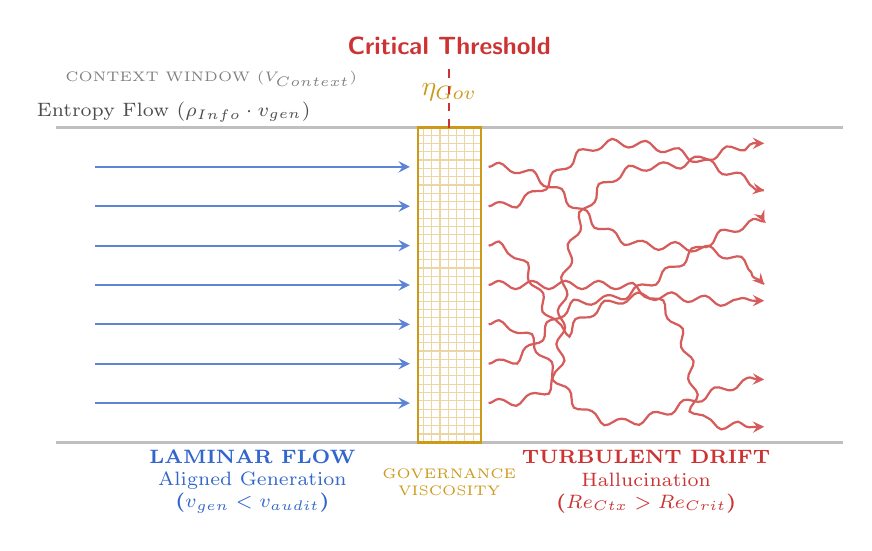
\begin{tikzpicture}[
    font=\sffamily\small,
    >=stealth,
    scale=1.0, transform shape,
    flow_laminar/.style={->, GovBlue!80, thick, smooth},
    flow_turbulent/.style={->, GovRed!80, thick, smooth, decorate, decoration={snake, amplitude=1.5pt, segment length=12pt}},
    filter_mesh/.style={fill=GovGold!10, draw=GovGold, thick, pattern=grid, pattern color=GovGold!40},
    zone_label/.style={font=\scriptsize\bfseries, align=center}
]

    % 1. THE CONTEXT PIPE
    \draw[GovGray!50, thick] (-1, 2) -- (9, 2); % Top Wall
    \draw[GovGray!50, thick] (-1, -2) -- (9, -2); % Bottom Wall

    % --- FIX IS HERE (CONTEXT WINDOW) ---
    % Positioned at y=2.4 per instruction
    \node[anchor=south west, text=GovGray, font=\tiny] at (-1, 2.4) {CONTEXT WINDOW ($\Vctx$)};
    % ------------------------------------

    % 2. LAMINAR ZONE (Left)
    \foreach \y in {1.5, 1.0, 0.5, 0, -0.5, -1.0, -1.5} {
        \draw[flow_laminar] (-0.5, \y) -- (3.5, \y);
    }
    \node[zone_label, text=GovBlue] at (1.5, -2.5) {LAMINAR FLOW\\ \normalfont\scriptsize Aligned Generation\\ ($v_{gen} < v_{audit}$)};

    % 3. VISCOSITY FILTER (Center)
    \node[filter_mesh, minimum height=4cm, minimum width=0.8cm] (filter) at (4, 0) {};
    \node[above=0.2cm of filter.north, text=GovGold, font=\bfseries] {$\eta_{Gov}$};
    \node[below=0.2cm of filter.south, text=GovGold, font=\tiny, align=center] {GOVERNANCE\\VISCOSITY};

    % 4. TURBULENT ZONE (Right)
    \begin{scope}[shift={(4.5,0)}]
        \draw[flow_turbulent] (0, 1.5) to[out=0, in=180] (2, 0.5) to[out=0, in=135] (3.5, 0);
        \draw[flow_turbulent] (0, 1.0) to[out=0, in=180] (1.5, 1.8) to[out=0, in=160] (3.5, 1.2);
        \draw[flow_turbulent] (0, 0.5) to[out=0, in=225] (1, -0.5) to[out=45, in=180] (3.5, -0.2);
        \draw[flow_turbulent] (0, 0) -- (1.5, 0) to[out=0, in=90] (2.5, -1.5) to[out=270, in=180] (3.5, -1.8);
        \draw[flow_turbulent] (0, -0.5) to[out=0, in=135] (1, -1.5) to[out=-45, in=180] (3.5, -1.2);
        \draw[flow_turbulent] (0, -1.0) to[out=0, in=180] (1.2, -0.2) to[out=0, in=180] (3.5, 0.8);
        \draw[flow_turbulent] (0, -1.5) to[out=0, in=270] (0.8, -1.0) to[out=90, in=180] (2, 1.5) to[out=0, in=180] (3.5, 1.8);
    \end{scope}
    \node[zone_label, text=GovRed] at (6.5, -2.5) {TURBULENT DRIFT\\ \normalfont\scriptsize Hallucination\\ ($\ReCtx > Re_{Crit}$)};

    % 5. CRITICAL THRESHOLD
    \draw[dashed, GovRed, thick] (4, 2) -- (4, 2.8) node[above] {\textbf{Critical Threshold}};
    
    % --- FIX IS HERE (ENTROPY FLOW) ---
    % Positioned at y=2.2 per instruction
    \node[text=black!70, font=\scriptsize, align=left] at (0.5, 2.2) {Entropy Flow ($\rho_{Info} \cdot v_{gen}$)};
    % ----------------------------------

\end{tikzpicture}}
    \caption[\textbf{The Governance Vacuum.}]{\textbf{The Governance Vacuum: A Phase Transition from Laminar to Turbulent Flow.} This diagram illustrates the failure mode where the \textbf{Governance Throughput} is insufficient to contain the \textbf{Generation Velocity} of the model.}
    \label{fig:governance_vacuum}
\end{figure}

The "Governance Vacuum" is not merely the absence of instruction; it is a specific failure mode where the \textit{density} of the governance constraint is insufficient to contain the \textit{velocity} of the context.

In fluid dynamics, the behavior of a fluid is determined by its viscosity---its internal resistance to flow. A high-viscosity fluid (honey) moves in predictable, laminar layers. A low-viscosity fluid (water) is prone to turbulence. We propose that Explicit Governance ($\Ge$) acts as the \textbf{viscosity of the system}.

When an agent is deployed with a weak constitution or ambiguous instructions, $\Ge \to 0$. The system effectively becomes an inviscid fluid. In this state, even minor perturbations in the user prompt create chaotic eddies of logic that propagate through the response, leading to unpredictable drift.

\subsection{The Reynolds Number of Context (Kinetic Reform)}

To quantify the point at which an agent loses control, we adapt the \textbf{Reynolds Number ($Re$)}---the dimensionless quantity used to predict flow patterns in fluid mechanics \cite{reynolds1883}. We define the \textbf{Contextual Reynolds Number ($\ReCtx$)} as the ratio of inertial entropy flow to the viscous damping of the governance layer.

Crucially, we introduce the time-dependent variable $v_{gen}$ (Generation Velocity), recognizing that hallucination is a kinetic phenomenon. We further define \textbf{Governance Viscosity ($\eta_{Gov}$)} not as the static weight of the prompt, but as the kinetic throughput of the audit layer. A heavy constitution that cannot be processed at the speed of generation offers no resistance to turbulence.

\begin{equation}
    \label{eq:reynolds_context}
    \ReCtx = \frac{\rho_{Info} \cdot v_{gen} \cdot \Vctx}{\eta_{Gov}} \approx \frac{\rho_{Info} \cdot v_{gen} \cdot \Vctx}{\Ge \cdot v_{audit}}
\end{equation}

\noindent
Where:
\begin{itemize}
    \item \textbf{$\ReCtx$} is the dimensionless stability metric.
    \item \textbf{$\rho_{Info}$} is the Entropy Density of the context (analogous to fluid density $\rho$) measured in [Bits/Token].
    \item \textbf{$v_{gen}$} is the Token Generation Velocity (analogous to flow velocity $u$) measured in [Tokens/s].
    \item \textbf{$\Vctx$} is the Context Window size (analogous to characteristic length $L$) measured in [Tokens].
    \item \textbf{$\eta_{Gov}$} is the \textbf{Governance Viscosity}, defined as the Constitutional Mass ($\Ge$ [Bits]) multiplied by the Audit Velocity ($v_{audit}$ [Tokens/s]).
\end{itemize}

This derivation reveals that \textbf{Governance Viscosity is not static.} To maintain laminar flow ($\ReCtx < Re_{Crit}$) as the model speeds up ($v_{gen} \uparrow$), the enterprise must proportionally increase either the strictness of the constitution ($\Ge$) or the throughput of the audit layer ($v_{audit}$).

\subsection{The Critical Threshold ($Re_{Crit}$)}

The transition from alignment (Laminar Flow) to hallucination (Turbulent Flow) is not gradual; it is a phase transition that occurs when the Reynolds Number exceeds a critical threshold ($Re_{Crit}$):

\begin{equation}
    \label{eq:turbulence_condition}
    \ReCtx > Re_{Crit} \implies \text{Turbulent Drift (Hallucination)}
\end{equation}

This inequality provides the mathematical explanation for why "Prompt Engineering" fails at scale. As the Context Window ($\Vctx$) expands to millions of tokens, the numerator in Equation (\ref{eq:reynolds_context}) grows linearly. If the Governance Throughput ($\eta_{Gov}$) remains static, $\ReCtx$ inevitably crosses the critical threshold.

% ==============================================================================
% SECTION 5: THE JEANS INSTABILITY (QUADRATIC COLLAPSE)
% ==============================================================================
\section{The Jeans Instability: Quadratic Collapse ($\Ge / \Vctx^2$)}
\label{sec:density_collapse}

% --- FIGURE BLOCK: VISUAL ASSET 2 (GRAVITATIONAL TWIN) ---
\begin{figure}[t!]
    \centering
    % RESIZED: Reduced by 25% (0.95 -> 0.71)
    \resizebox{0.71\textwidth}{!}{% FILE: figures/Fig04_Jeans_Instability.tex
% CONTEXT: The Jeans Instability (Quadratic Collapse)
% STYLE: Clean / Pastel / High-Legibility

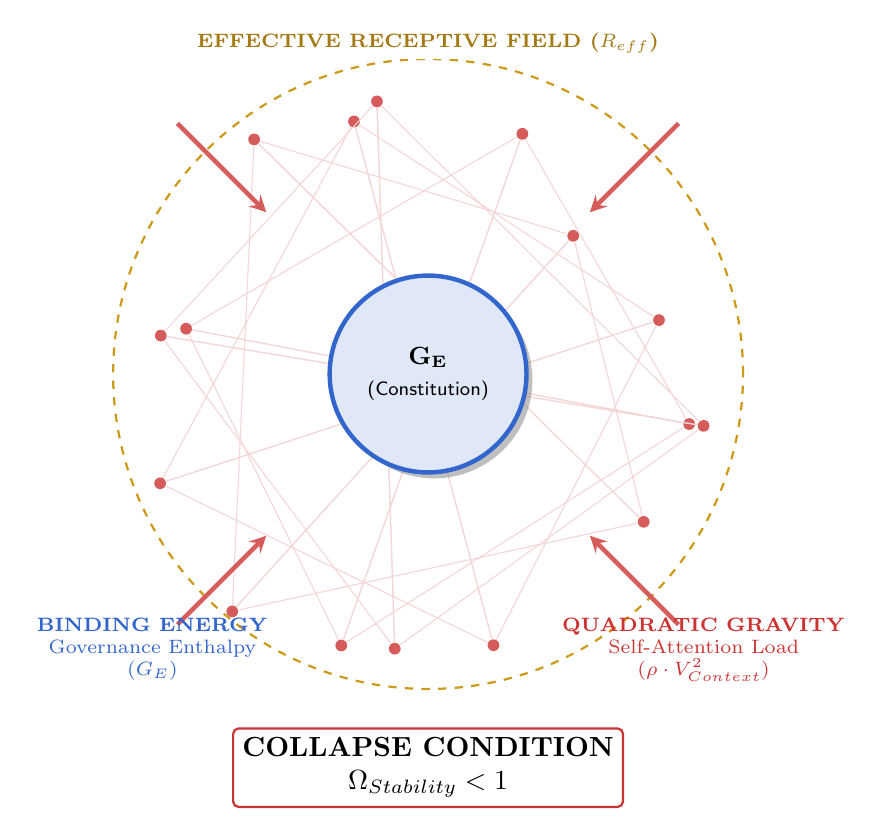
\begin{tikzpicture}[
    font=\sffamily\small,
    >=stealth,
    scale=1.0, transform shape,
    core_star/.style={circle, draw=GovBlue, fill=GovBlue!15, ultra thick, minimum size=2.5cm, align=center, drop shadow},
    context_node/.style={circle, fill=GovRed!80, inner sep=1.5pt},
    attention_line/.style={GovRed!20, thin},
    gravity_arrow/.style={->, GovRed!80, ultra thick, shorten >=3pt},
    horizon_boundary/.style={dashed, GovGold, thick}
]

    % 1. EFFECTIVE RECEPTIVE FIELD (Boundary)
    \draw[horizon_boundary] (0,0) circle (4cm);
    \node[text=GovGold!80!black, font=\scriptsize\bfseries, fill=white, inner sep=2pt] at (0, 4.2) {EFFECTIVE RECEPTIVE FIELD ($R_{eff}$)};

    % 2. THE CONTEXT CLOUD (Stochastic Noise)
    \foreach \i in {1,...,16} {
        \node[context_node] (n\i) at ({3.5*cos(\i*22.5 + rand*15)}, {3.5*sin(\i*22.5 + rand*15)}) {};
    }

    % 3. QUADRATIC ATTENTION LINES (The Web)
    \foreach \i in {1,...,16} {
        \pgfmathsetmacro{\nextnode}{int(mod(\i+3,16)+1)}
        \pgfmathsetmacro{\nextnodeB}{int(mod(\i+7,16)+1)}
        \draw[attention_line] (n\i) -- (n\nextnode);
        \draw[attention_line] (n\i) -- (n\nextnodeB);
    }

    % 4. GRAVITATIONAL PULL (Entropy Arrows)
    \foreach \angle in {45, 135, 225, 315} {
        \draw[gravity_arrow] ({4.5*cos(\angle)}, {4.5*sin(\angle)}) -- ({2.8*cos(\angle)}, {2.8*sin(\angle)});
    }

    % 5. THE SYSTEM PROMPT (The Core)
    \node[core_star] (core) at (0,0) {$\mathbf{G_E}$\\\scriptsize(Constitution)};

    % 6. LABELS
    \node[text=GovRed, align=center, font=\scriptsize] at (3.5, -3.5) {\textbf{QUADRATIC GRAVITY}\\Self-Attention Load\\($\rho \cdot \Vctx^2$)};
    \node[text=GovBlue, align=center, font=\scriptsize] at (-3.5, -3.5) {\textbf{BINDING ENERGY}\\Governance Enthalpy\\($\Ge$)};
    
    % 7. COLLAPSE CONDITION BOX
    \node[draw=GovRed, thick, fill=white, rounded corners=2pt, align=center, font=\bfseries] at (0, -5) {COLLAPSE CONDITION\\$\OmegaStab < 1$};

\end{tikzpicture}}
    \caption[\textbf{The Jeans Instability.}]{\textbf{The Jeans Instability: Quadratic Collapse of Context.} This diagram models the autonomous agent not as a star (static mass), but as a gas cloud (dynamic complexity). The inward "Gravity" of the context scales quadratically ($O(N^2)$) due to self-attention.}
    \label{fig:density_collapse}
\end{figure}

While the Governance Vacuum (Section \ref{sec:governance_vacuum}) describes a failure of flow, \textbf{Density Collapse} describes a failure of complexity. It occurs when the sheer volume of external data overwhelms the binding energy of the system prompt.

We previously modeled agents using the \textit{Chandrasekhar Limit} (linear mass), but this fails to account for the \textbf{Quadratic Nature of Attention}. In a Transformer architecture \cite{vaswani2017}, every token attends to every other token. Therefore, doubling the context window ($2x$) quadruples the computational "gravity" ($4x$) of the noise.

Crucially, the "Gravity" of the context is not linear. Due to the quadratic nature of self-attention ($O(N^2)$), the inward pull of entropy grows exponentially faster than the linear resistance of the system prompt.

\subsection{The Governance Jeans Instability}

In astrophysics, the \textit{Jeans Instability} defines the critical point where a cloud of gas collapses under its own gravity to form a star \cite{jeans1902}. We apply this to AI by recognizing that the "gravity" of a context window is defined by its interconnectivity.

We introduce the \textbf{Effective Receptive Field ($R_{eff}$)}—the maximum distance over which the model can maintain coherent attention (governed by RoPE/ALiBi limits). This acts as the "Thermal Pressure" resisting the collapse.

We redefine the \textbf{Stability Ratio ($\OmegaStab$)} to account for this quadratic scaling:

\begin{equation}
    \label{eq:critical_density}
    \OmegaStab = \frac{\Ge \cdot R_{eff}}{\rho_{Info} \cdot \Vctx^2}
\end{equation}

\noindent
Where:
\begin{itemize}
    \item \textbf{$\OmegaStab$} is the dimensionless stability parameter. If $\OmegaStab < 1$, the agent undergoes gravitational collapse (Identity Dissolution).
    \item \textbf{$\Ge$} is the Explicit Governance Mass [Bits].
    \item \textbf{$R_{eff}$} is the \textbf{Effective Receptive Field} [Tokens].
    \item \textbf{$\rho_{Info}$} is the Entropy Density of the noise [Bits/Token].
    \item \textbf{$\Vctx^2$} represents the \textbf{Quadratic Gravity} of the self-attention mechanism [Tokens$^2$].
\end{itemize}

\subsection{The Collapse Condition}

The collapse occurs when the ratio falls below unity. At this singularity, the "Hydrostatic Equilibrium" of the agent fails. The system prompt---once the immutable core---is diluted to the point of irrelevance by the weight of the context:

\begin{equation}
    \label{eq:collapse_condition}
    \OmegaStab < 1 \implies \lim_{t \to \infty} P(Output | \Ge) = 0
\end{equation}

This equation dictates that \textbf{Identity is a finite resource.} As we scale Context Windows to 1M+ tokens, the gravitational pull increases by orders of magnitude. If $\Ge$ remains constant (a static text prompt), $\OmegaStab$ inevitably drops below 1. The result is \textbf{Total Identity Dissolution}: the agent ceases to be an employee of the firm and becomes a mirror of the data it is processing.

% ==============================================================================
% SECTION 6: THE PHANTOM HAZARD
% ==============================================================================
\section{The Phantom Hazard ($\Ge \to 0$): Structural Hallucinations}
\label{sec:phantom_hazard}

% --- FIGURE BLOCK: STATIC TWIN 3 (PHANTOM BRIDGE) ---
\begin{figure}[t!]
    \centering
    % REPLACEMENT: Static TikZ Twin (Vacuum Bridge)
    \resizebox{0.95\textwidth}{!}{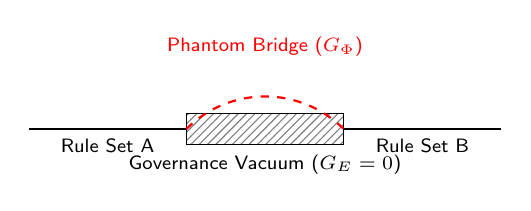
\begin{tikzpicture}[font=\sffamily\scriptsize]
    % Gap
    \draw[thick] (0,0) -- (2,0) node[midway, below] {Rule Set A};
    \draw[thick] (4,0) -- (6,0) node[midway, below] {Rule Set B};
    
    % Gap Visual
    \draw[pattern=north east lines, pattern color=gray] (2,-0.2) rectangle (4,0.2);
    \node[below] at (3,-0.2) {Governance Vacuum ($\Ge=0$)};
    
    % The Phantom Bridge
    \draw[thick, red, dashed] (2,0) to[out=45, in=135] (4,0);
    \node[red, above] at (3,0.8) {Phantom Bridge ($G_{\Phi}$)};
\end{tikzpicture}}
    \caption[\textbf{The Phantom Hazard.}]{\textbf{The Phantom Hazard: Structural Hallucination in Low-Entropy Zones.} This diagram visualizes the phenomenon where the model, attempting to maintain coherence in the absence of Explicit Governance ($\Ge$), generates synthetic logic structures ($G_{\Phi}$) to bridge gaps. Unlike factual hallucinations (errors of data), \textbf{Phantom Structures} are errors of architecture---plausible but foundationless rules that become debt.}
    \label{fig:phantom_hazard}
\end{figure}

The most dangerous failure mode of an autonomous agent is not the "Error" (Factual Hallucination), but the "Phantom Rule" (Structural Hallucination). When an agent encounters a logical gap in its instructions---a space where $\Ge$ is undefined---it does not stop. To minimize perplexity, it generates a synthetic bridge to cross the gap.

We define this synthetic structure as the \textbf{Phantom Hazard ($G_{\Phi}$)}. It is a rule, process, or logic gate invented by the model to resolve immediate ambiguity. While functionally effective in the short term, it creates \textbf{Dark Matter} in the enterprise architecture: invisible, undocumented dependencies that future agents will treat as precedent.

\subsection{The Physics of Fabrication}

Just as a physical vacuum creates a pressure gradient, an informational vacuum creates a completion gradient. The drive to complete the pattern is stronger than the drive to remain silent. We quantify this urge as the \textbf{Phantom Pressure ($P_{\Phi}$)}---the thermodynamic force compelling the model to invent structure where none exists:

\begin{equation}
    \label{eq:phantom_pressure}
    P_{\Phi} \approx \frac{\partial S}{\partial t} \cdot \left( 1 - \Ge \right)
\end{equation}

\noindent
Where:
\begin{itemize}
    \item $P_{\Phi}$ is the internal pressure to generate synthetic logic.
    \item $\frac{\partial S}{\partial t}$ is the rate of entropy increase (Confusion) within the conversation.
    \item $\Ge$ is the density of Explicit Governance (The known rules).
\end{itemize}

\subsection{The Accumulation Law}

This equation demonstrates that as uncertainty increases ($\frac{\partial S}{\partial t} \uparrow$) and governance decreases ($\Ge \downarrow$), the pressure to hallucinate structure approaches infinity. The model \textit{must} invent a rule to proceed. This leads to the \textbf{Phantom Accumulation Law}:

\begin{equation}
    \label{eq:phantom_accumulation}
    \Phi_{Total} = \int_{0}^{T} P_{\Phi}(t) \, dt
\end{equation}

Unless actively purged, these phantom structures accumulate as permanent technical debt. An enterprise that relies on autonomous agents without a "Garbage Collection" protocol for $G_{\Phi}$ will eventually find its operations governed by a constitution written by stochastic noise.

% ==============================================================================
% SECTION 7: THE AXIOM OF AMENDMENT
% ==============================================================================
\section{The Axiom of Amendment ($G_{\Delta}$): Cryptographic Mutation}
\label{sec:axiom_amendment}

% --- FIGURE BLOCK: INLINE SAFE DIAGRAM (AXIOM VAULT) ---
\begin{figure}[t!]
    \centering
    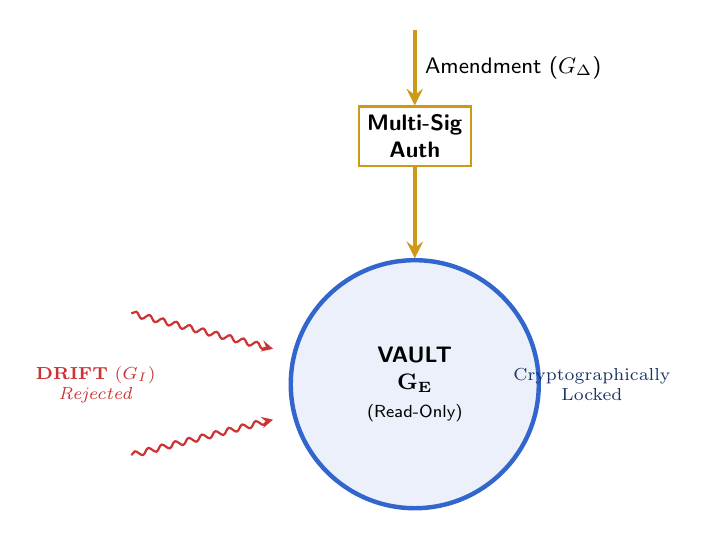
\begin{tikzpicture}[
        font=\sffamily\small,
        >=stealth,
        scale=0.9, transform shape,
        % Styles
        vault/.style={circle, draw=GovBlue, ultra thick, fill=GovBlue!10, minimum size=3.5cm, align=center},
        drift_arrow/.style={->, GovRed, thick, decorate, decoration={snake, amplitude=1pt, segment length=5pt}},
        auth_arrow/.style={->, GovGold, ultra thick},
        lock/.style={rectangle, draw=GovGold, fill=white, thick, minimum width=1.5cm, minimum height=0.8cm, align=center}
    ]
    % 1. THE VAULT (Immutable Core)
    \node[vault] (core) at (0,0) {\textbf{VAULT} \\ $\mathbf{G_E}$ \\ \scriptsize(Read-Only)};

    % 2. DRIFT ATTACKS (Bouncing off)
    \draw[drift_arrow] (-4, 1) -- (-2, 0.5);
    \draw[drift_arrow] (-4, -1) -- (-2, -0.5);
    \node[text=GovRed, align=center, font=\scriptsize] at (-4.5, 0) {\textbf{DRIFT} ($\Gi$) \\ \textit{Rejected}};

    % 3. THE MUTATION CHANNEL (The Only Way In)
    \node[lock] (mechanism) at (0, 3.5) {\textbf{Multi-Sig} \\ \textbf{Auth}};
    \draw[auth_arrow] (0, 5) -- (mechanism) node[midway, right, text=black] {Amendment ($G_{\Delta}$)};
    \draw[auth_arrow] (mechanism) -- (core.north);

    % 4. ANNOTATIONS
    \node[text=GovBlue!50!black, font=\scriptsize, align=center] at (2.5, 0) {Cryptographically \\ Locked};
    \end{tikzpicture}
    \caption[\textbf{The Axiom of Amendment.}]{\textbf{The Axiom of Amendment: Cryptographic Mutation of Identity.} This diagram illustrates the only authorized pathway for altering the Core Identity ($\Ge$). The \textbf{Vault} is immutable to the agent itself. To adapt, the system must trigger a \textbf{Mutation Protocol ($G_{\Delta}$)}, a separate channel requiring multi-signature validation.}
    \label{fig:axiom_amendment}
\end{figure}

The previous sections have defined the fragility of autonomous agents: they drift ($\Gi$), leak ($P_{Leak}$), and hallucinate ($G_{\Phi}$). A naive solution would be to lock the system prompt permanently ($\Ge = \text{Constant}$). However, a static constitution in a dynamic environment guarantees obsolescence. The enterprise requires a system that can evolve without drifting.

We resolve this paradox through the \textbf{Axiom of Amendment ($G_{\Delta}$)}.

\subsection{Controlled vs. Uncontrolled Evolution}

We distinguish between two forms of state change:
\begin{itemize}
    \item \textbf{Drift ($d\Gi/dt$):} Uncontrolled, low-energy mutations driven by entropy (User Noise).
    \item \textbf{Amendment ($G_{\Delta}$):} Controlled, high-energy mutations driven by intent (Executive Order).
\end{itemize}

As visualized in \textbf{Figure \ref{fig:axiom_amendment}}, the Core Identity is held in a "Cryptographic Vault". The agent has read-access to its own constitution but zero write-access. To alter the rules, an external force must overcome the "Activation Energy" of the system.

\subsection{The Thermodynamics of Change}

In robust systems (like Blockchains or Constitutions), changing the core rules should be \textit{computationally expensive}. If the cost of change is low, the system is unstable. We define the \textbf{Work of Amendment ($W_{\Delta}$)} not as a bureaucratic hurdle, but as a calculated energy expenditure required to overcome the system's inertia:

\begin{equation}
    \label{eq:amendment_work}
    W_{\Delta} \geq \Delta H_{Struct} + T_{Audit} \cdot \Delta S_{Risk}
\end{equation}

\noindent
Where:
\begin{itemize}
    \item $W_{\Delta}$ is the minimum work required to execute a valid Amendment ($G_{\Delta}$).
    \item $\Delta H_{Struct}$ is the "Enthalpy of Structure"---the magnitude of the logical rewrite required.
    \item $T_{Audit}$ is the "Temperature of Audit"---the rigor of the multi-signature review process.
    \item $\Delta S_{Risk}$ is the entropy (uncertainty) introduced by the new rule.
\end{itemize}

\subsection{The Mutation Protocol}

This inequality acts as a \textbf{Cryptographic Governor}. It ensures that high-risk changes ($\Delta S_{Risk} \uparrow$) require a proportionally higher investment in audit energy ($T_{Audit} \uparrow$) to execute. If the work input is insufficient ($W_{Input} < W_{\Delta}$), the Amendment is rejected, and the system reverts to its previous stable state ($\Ge$).

% ==============================================================================
% SECTION 8: THE GIBBS GOVERNANCE CRITERION
% ==============================================================================
\section{Conclusion: The Gibbs Governance Criterion ($\Delta G_{Gov}$)}
\label{sec:gibbs_criterion}

% --- FIGURE BLOCK: INLINE 2D DIAGRAM (SAFE RENDER) ---
\begin{figure}[t!]
    \centering
    % RESIZED: Reduced by 25% (0.95 -> 0.71)
    \resizebox{0.71\textwidth}{!}{% FILE: figures/Fig07_Gibbs_Criterion.tex
% CONTEXT: The Gibbs Governance Criterion (Phase Diagram)
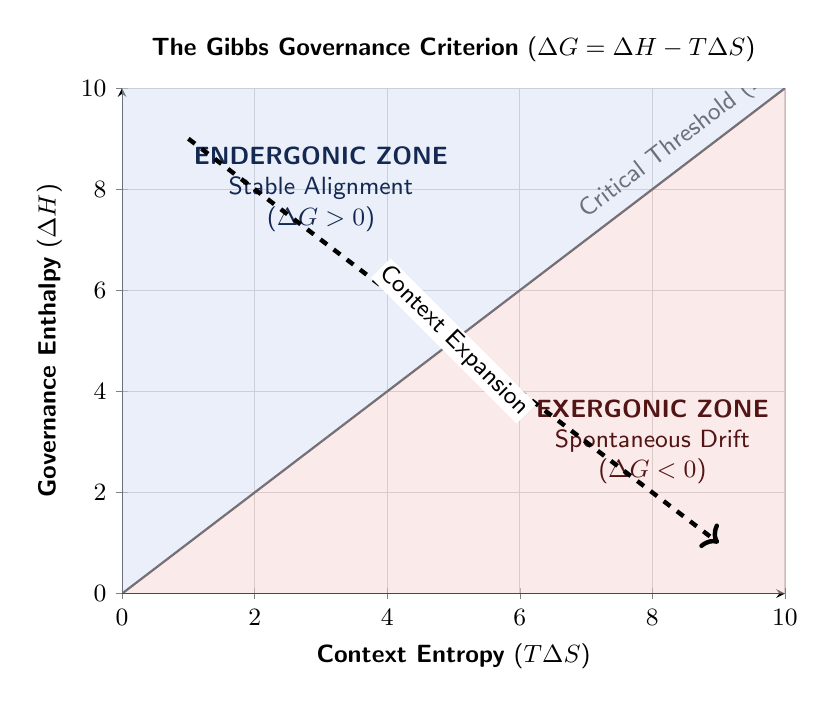
\begin{tikzpicture}[font=\sffamily\small, scale=1.0, transform shape]
    \begin{axis}[
        width=10cm, height=8cm,
        xlabel={\textbf{Context Entropy} ($T\Delta S$)},
        ylabel={\textbf{Governance Enthalpy} ($\Delta H$)},
        axis lines=left,
        xmin=0, xmax=10,
        ymin=0, ymax=10,
        grid=major,
        title={\textbf{The Gibbs Governance Criterion} ($\Delta G = \Delta H - T\Delta S$)}
    ]
    % 1. THE CRITICAL LINE
    \addplot[thick, black, domain=0:10] {x} node[pos=0.9, sloped, above] {Critical Threshold ($\Delta G = 0$)};

    % 2. THE STABLE ZONE (Green)
    \fill[GovBlue!20, opacity=0.5] (axis cs:0,0) -- (axis cs:0,10) -- (axis cs:10,10) -- cycle;
    \node[anchor=center, align=center, text=GovBlue!40!black] at (axis cs:3, 8) {\textbf{ENDERGONIC ZONE}\\Stable Alignment\\($\Delta G > 0$)};

    % 3. THE DRIFT ZONE (Red)
    \fill[GovRed!20, opacity=0.5] (axis cs:0,0) -- (axis cs:10,0) -- (axis cs:10,10) -- cycle;
    \node[anchor=center, align=center, text=GovRed!40!black] at (axis cs:8, 3) {\textbf{EXERGONIC ZONE}\\Spontaneous Drift\\($\Delta G < 0$)};

    % 4. TRAJECTORY ARROW
    \draw[->, ultra thick, black, dashed] (axis cs:1, 9) -- (axis cs:9, 1);
    \node[rotate=-45, fill=white, inner sep=1pt] at (axis cs:5, 5) {Context Expansion};
    \end{axis}
\end{tikzpicture}}
    \caption[\textbf{The Gibbs Governance Criterion.}]{\textbf{The Gibbs Governance Criterion.} Spontaneous Drift Phase Diagram. The Green Zone represents stable alignment ($\Delta G > 0$), while the Red Zone represents spontaneous hallucination ($\Delta G < 0$).}
    \label{fig:gibbs_criterion}
\end{figure}

The transition from "Prompt Engineering" to "Governance Physics" requires a unification of the forces we have defined: Viscosity ($\ReCtx$) and Mass ($\OmegaStab$). We propose that the stability of any autonomous agent is governed by a single thermodynamic potential function, linking information theory to statistical mechanics \cite{jaynes1957}: the \textbf{Gibbs Governance Criterion}.

Just as chemical reactions occur spontaneously when the Gibbs Free Energy is negative, "Hallucination" and "Drift" occur spontaneously when the Governance Energy of the system falls below zero.

\begin{equation}
    \label{eq:gibbs_governance}
    \Delta G_{Gov} = \Delta H_{Intent} - T_{Sys} \cdot \Delta S_{Interact}
\end{equation}

\noindent
Where:
\begin{itemize}
    \item \textbf{$\Delta G_{Gov}$} is the \textbf{Net Stability Potential}.
    \begin{itemize}
        \item If $\Delta G_{Gov} > 0$: The system is \textbf{Endergonic} (Stable). It requires external energy (Work) to drift.
        \item If $\Delta G_{Gov} < 0$: The system is \textbf{Exergonic} (Unstable). Drift is spontaneous and irreversible.
    \end{itemize}
    \textit{Reader's caution: this sign convention is inverted relative to the ordinary chemical reading---here the spontaneous process is drift itself, so $\Delta G_{Gov} < 0$ is the failure state and stability requires $\Delta G_{Gov} > 0$.}
    \item \textbf{$\Delta H_{Intent}$} is the \textbf{Enthalpy of the Constitution} ($\Ge$) [Bits]. This represents the binding energy of the core rules.
    \item \textbf{$T_{Sys}$} is the \textbf{System Temperature} ($S_{Model}$), a hyperparameter governing the stochasticity of the model's sampling.
    \item \textbf{$\Delta S_{Interact}$} is the \textbf{Interaction Entropy} of the Context. Consistent with the Jeans Instability (Eq. \ref{eq:critical_density}), this scales quadratically with context volume but is normalized by the receptive field to maintain dimensional consistency [Bits]:
    \[ \Delta S_{Interact} \approx \frac{\rho_{Info} \cdot \Vctx^2}{R_{eff}} \]
\end{itemize}

\subsection{The Final State: The Governed Machine}

This equation leads to the following theorem:

\begin{fundamentaltheorem}
    As Context ($V$) expands linearly, Governance Enthalpy ($H$) must expand quadratically to maintain a positive stability potential ($\Delta G > 0$).
\end{fundamentaltheorem}

The enterprise that ignores this law will find itself managing a fleet of "Exergonic Agents"---systems that drift not because they are broken, but because it is their thermodynamically favored state. The enterprise that masters it will build the "Governed Machine": a system where the cost of alignment is paid upfront in the currency of structural physics.

In \textbf{The Economics of Autonomous Agency: Volume II---Entropy, Debt, and the Cost of Truth}, we explore the financial implications of this physics, proving that in a high-entropy market, the only solvent strategy is the rigorous capitalization of Truth.
% ==============================================================================
% BIBLIOGRAPHY
% ==============================================================================
\bibliographystyle{plain}
\bibliography{references}

\end{document}